
\chapter{FCR Units}
\raggedbottom

Most medium and heavy AAA batteries can be associated with an add-on fire-control radar (FCR), which improves their accuracy and allows them to engage unsighted targets at night and in adverse weather. These units are presented below with their counters.

% \begin{figure}[ht]
%     \centering
%     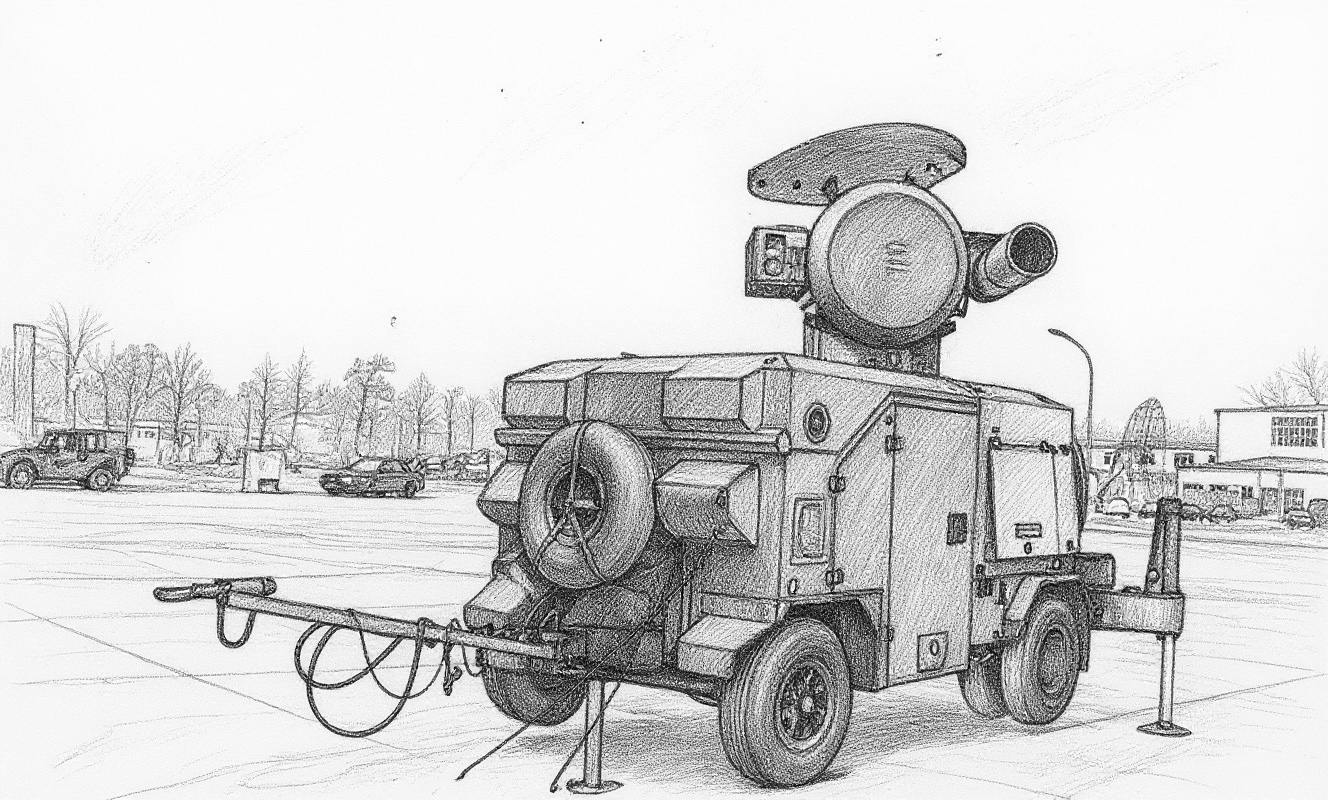
\includegraphics[width=\linewidth]{photos/skyguard.jpg}
%     % https://commons.wikimedia.org/wiki/File:Skyguard.jpg
% \end{figure}

The \hyperlink{table:fcr-units}{FCR Unit Table} summarizes the properties of FCR units.
As well as the basic properties common to all ground units, the table gives:
the FCR class;
the frequency band; and
the modifier to the hit roll.

\subsectionwithcounter{Towed FCR-A Platoon}{\counter{towed FCR-A platoon}}{
    FCR-As typically use 1940s technology. They include the SON-9 FCR.
}

\paragraphwithcounter{SON-9}{}{
    The Soviet SON-9 (Fire Can) FCR-A was derived from the earlier SON-4, which in turn was derived from the US-supplied SCR-584.
    It is commonly used with 57~mm S-60, 85~mm KS-12, 100~mm KS-19, and 130~mm KS-30 batteries.

    The SON-9 entered service in 1955 with Soviet forces and was widely exported to Soviet allies.
    It has seen combat, including with North Vietnam in the Vietnam War, Egypt and Syria in the 1967 War, the War of Attrition, and the 1973 War.%
    \note{SON-9}{
        Wikipedia states this was used with the 57, 85, 100, and 130~mm guns and was widely deployed in the Vietnam War. In {\TSOH} the 57~mm S-60 and 85~mm KS-12 are often combined with a FCR-A, presumably the SON-9. The service history is from Wikipedia.
    }

}

\subsectionwithcounter{Towed FCR-B Platoon}{\counter{towed FCR-B platoon}}{
    FCR-Bs typically use 1950s technology.
}

\subsectionwithcounter{Towed FCR-C Platoon}{\counter{towed FCR-C platoon}}{
    FCR-Cs typically use 1960s technology.
    They include the Super Fledermaus and Flycatcher FCRs.
}

\paragraphwithcounter{Super Fledermaus}{}{
    The Contraves Super Fledermaus FCR-C can control a section of two Oerlikon GDF 35~mm guns; it cannot control a whole battery.

    It entered service in 1965 with the Swiss Air Force and also was used by the Argentine Air Force, Brazil, Iran, Japan, and South Africa.
    It saw combat in the 1982 South Atlantic War in the defense of BAM Malvinas (Port Stanley Airport).%
    \note{Super Fledermaus}{
        Wikipedia states there were two versions: the Feuerleitgerät (FLt Gt) 63 (from 1965) and the Feuerleitgerät 69 (from 1970). The latter had “background clutter suppression,” which probably is equivalent to MTI.

        Wikipedia also states these the prototype of the Gepard used a Flt Gt 63. Since the FCR-W radar of the Gepard is equivalent to a \plus{2} modifier and has VF frequency, it corresponds to an FCR-C. We assume the Super Fledermaus does too.

    }
}
\paragraphwithcounter{Flycatcher}{}{
    The Signaal Flycatcher FCR-C can control up to six Bofors L/60 or L/70 guns or SAM launchers.

    Flycatcher entered service with the Royal Netherlands Air Force in 1979. It subsequently served with the Indian Armed Forces from 1985, the Irish Defense Forces from 2003, the Royal Netherlands Army from 1987, the Thai Armed Forces from 1981, Turkey, and Venezuela.%
    \note{Flycatcher}{
        Flycatcher is similar to the Cheetah radar, so presumably FCR-C.

        Sources: \href{https://en.wikipedia.org/wiki/Flycatcher_(radar)}{Wikipedia} and \href{https://magazines.defensie.nl/materieelgezien/2020/09/06_flycatche}{Terug naar de toekomst: De Flycatcher}.
    }
}

\subsectionwithcounter{Towed FCR-D Platoon}{\counter{towed FCR-D platoon}}{
    FCR-Ds typically use 1970s technology.
    The include the Skyguard.
}

\paragraphwithcounter{Skyguard}{}{
    The Contraves Skyguard FCR-D can control two Oerlikon GDF 35~mm guns and additionally a SAM launcher with AIM-9 Sparrow, RIM-9 Sea Sparrow, or Aspide missiles.

    Skyguard entered service in 1977 with the Swiss Air Force.
    It was subsequently very widely exported and used by the Argentine Army, Austria, Bahrain, Bangladesh, Brazil, Canada, Chile, China, Cyprus, Egypt, Greece, Indonesia, Iran, Italy, South Korea, Kuwait, Malaysia, Oman, Pakistan, Saudi Arabia, Spain, Taiwan, and the UK.
    It saw combat with the Argentine Army in the 1982 South Atlantic War in the defense of BAM Malvinas (Port Stanley Airport) and BAM Condor (Goose Green Airfield).
}

\begin{table}
    \caption*{\hypertarget{table:fcr-units}{FCR Unit Table}}
    \centering
    \footnotesize
    \input{table-fcr-units.tex}
    \label{table:fcr-units}
\end{table}
